%%\documentclass[a4paper,12pt,oneside]{llncs}
\documentclass[12pt,letterpaper]{article}
\usepackage[right=2cm,left=3cm,top=2cm,bottom=2cm,headsep=0cm]{geometry}

%%%%%%%%%%%%%%%%%%%%%%%%%%%%%%%%%%%%%%%%%%%%%%%%%%%%%%%%%%%
%% Juego de caracteres usado en el archivo fuente: UTF-8
\usepackage{ucs}
\usepackage[utf8x]{inputenc}

%%%%%%%%%%%%%%%%%%%%%%%%%%%%%%%%%%%%%%%%%%%%%%%%%%%%%%%%%%%
%% Juego de caracteres usado en la salida dvi
%% Otra posibilidad: \usepackage{t1enc}
\usepackage[T1]{fontenc}

%%%%%%%%%%%%%%%%%%%%%%%%%%%%%%%%%%%%%%%%%%%%%%%%%%%%%%%%%%%
%% Ajusta maergenes para a4
%\usepackage{a4wide}

%%%%%%%%%%%%%%%%%%%%%%%%%%%%%%%%%%%%%%%%%%%%%%%%%%%%%%%%%%%
%% Uso fuente postscript times, para que los ps y pdf queden y pequeños...
\usepackage{times}

%%%%%%%%%%%%%%%%%%%%%%%%%%%%%%%%%%%%%%%%%%%%%%%%%%%%%%%%%%%
%% Posibilidad de hipertexto (especialmente en pdf)
%\usepackage{hyperref}
\usepackage[bookmarks = true, colorlinks=true, linkcolor = black, citecolor = black, menucolor = black, urlcolor = black]{hyperref}

%%%%%%%%%%%%%%%%%%%%%%%%%%%%%%%%%%%%%%%%%%%%%%%%%%%%%%%%%%%
%% Graficos 
\usepackage{graphics,graphicx}

%%%%%%%%%%%%%%%%%%%%%%%%%%%%%%%%%%%%%%%%%%%%%%%%%%%%%%%%%%%
%% Ciertos caracteres "raros"...
\usepackage{latexsym}

%%%%%%%%%%%%%%%%%%%%%%%%%%%%%%%%%%%%%%%%%%%%%%%%%%%%%%%%%%%
%% Matematicas aun más fuertes (american math dociety)
\usepackage{amsmath}

%%%%%%%%%%%%%%%%%%%%%%%%%%%%%%%%%%%%%%%%%%%%%%%%%%%%%%%%%%%
\usepackage{multirow} % para las tablas
\usepackage[spanish,es-tabla]{babel}

%%%%%%%%%%%%%%%%%%%%%%%%%%%%%%%%%%%%%%%%%%%%%%%%%%%%%%%%%%%
%% Fuentes matematicas lo mas compatibles posibles con postscript (times)
%% (Esto no funciona para todos los simbolos pero reduce mucho el tamaño del
%% pdf si hay muchas matamaticas....
\usepackage{mathptm}

%%% VARIOS:
%\usepackage{slashbox}
\usepackage{verbatim}
\usepackage{array}
\usepackage{listings}
\usepackage{multirow}

%% MARCA DE AGUA
%% Este package de "draft copy" NO funciona con pdflatex
%%\usepackage{draftcopy}
%% Este package de "draft copy" SI funciona con pdflatex
%%%\usepackage{pdfdraftcopy}
%%%%%%%%%%%%%%%%%%%%%%%%%%%%%%%%%%%%%%%%%%%%%%%%%%%%%%%%%%%
%% Indenteacion en español...
\usepackage[spanish]{babel}

\usepackage{listings}
% Para escribir código en C
% \begin{lstlisting}[language=C]
% #include <stdio.h>
% int main(int argc, char* argv[]) {
% puts("Hola mundo!");
% }
% \end{lstlisting}


\title{ConvolucionAnalisis}
\author{Jesús Rodríguez Heras}

\begin{document}
	
	\maketitle
	\begin{abstract} %Poner esto en todas las prácticas de PCTR
		\begin{center}
			Resultados obtenidos en la comparación de Java y C++ en sus versiones secuencial y paralela en la convolución de una imagen.
		\end{center}
	\end{abstract}
	\thispagestyle{empty}
	\newpage
	
%	\tableofcontents
%	\newpage
	
	%%\listoftables
	%%\newpage
	
	%%\listoffigures
	%%\newpage
	
	%%%% REAL WORK BEGINS HERE:
	
	%%Configuracion del paquete listings
	\lstset{language=bash, numbers=left, numberstyle=\tiny, numbersep=10pt, firstnumber=1, stepnumber=1, basicstyle=\small\ttfamily, tabsize=1, extendedchars=true, inputencoding=latin1}

\section{Linux}
\subsection{Tiempo}
\begin{figure}[h]
	\centering
	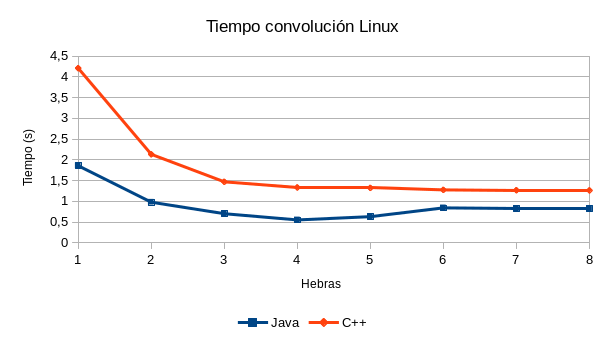
\includegraphics[scale=0.8]{TiempoLinux.png}
\end{figure}
\subsection{Speed-Up}
\begin{figure}[h]
	\centering
	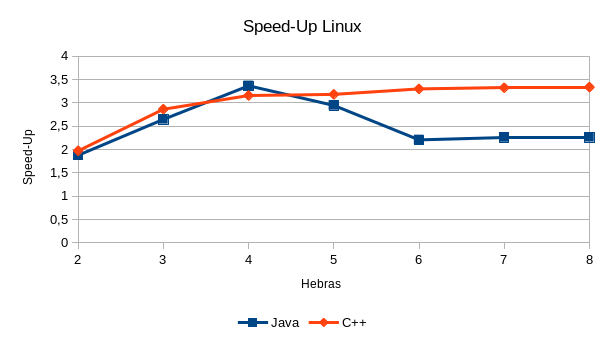
\includegraphics[scale=0.8]{SpeedUpLinux.png}
\end{figure}
\newpage

\section{Windows}
\subsection{Tiempo}
%\begin{figure}[h]
%	\centering
%	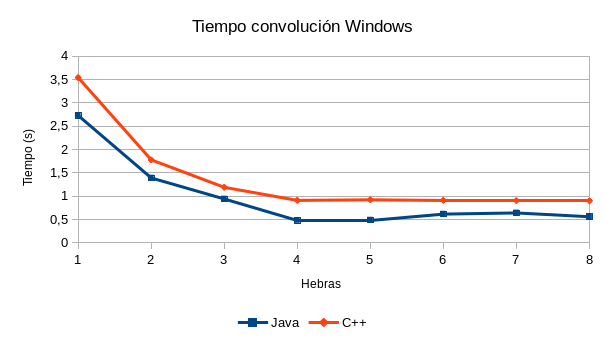
\includegraphics[scale=1]{TiempoWindows.png}
%\end{figure}
\subsection{Speed-Up}
%\begin{figure}[h]
%	\centering
%	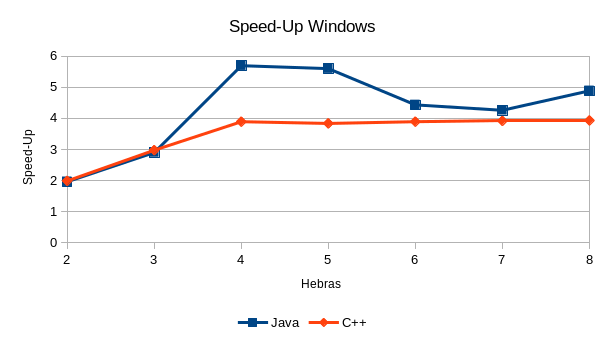
\includegraphics[scale=1]{SpeedUpWindows.png}
%\end{figure}

\section{Conclusión}
La conclusión general que podemos obtener de esta práctica es que, en Java, el mejor número de hebras es aquel que se corresponde con los cores de la máquina en la que se está ejecutando la aplicación, debido a que, un número excesivo de hebras, conllevará un aumento del tiempo de ejecución. Sin embargo, en C++, podemos observar como el Speed-Up sigue en aumento con un número mayor de hebras.

Por el contrario, Java es más rápido que C++ en el proceso de convolución de una imagen, tal como se puede observar en los gráficos anteriores\footnote{Para estos gráficos se han realizado pruebas en una máquina con procesador Intel i5-3570 CPU @ 3.40GHz × 4, tanto en Linux (Debian 9.6), como en Windows (cuenta con dual-boot a ambos sistemas operativos). Se ha seleccionado el filtro de ``enfoque'' para todas las pruebas realizadas para que sean lo más realistas posibles.}.


\end{document}